% Usar el tipo de documento: Artículo científico.
\documentclass[12pt,a4paper]{article}

% Cargar mensajes en español.
\usepackage[spanish]{babel}

% Usar codificación utf-8 para acentos y otros.
\usepackage[utf8]{inputenc}

%Dimensiones de los márgenes.
\usepackage[margin=1.5cm]{geometry}

% Insertar porciones de código
\usepackage{listings}

% Comenzar párrafos con separación no indentación.
\usepackage{parskip}

% Usar gráficos
\usepackage{graphicx}
\usepackage{caption}
\usepackage{subcaption}
%
% Usar contenedores flotantes para figuras.
\usepackage{float}

% Carpeta de las imágenes.
\graphicspath{{img/}}

% Configuración para porciones de código.
\lstset{
%	language=bash,
	basicstyle=\ttfamily\small,
%	numberstyle=\footnotesize,
%	numbers=left,
%	backgroundcolor=\color{gray!10},
%	frame=single,
	tabsize=4,
%	rulecolor=\color{black!30},
%	title=\lstname,
%	escapeinside={\%*}{*)},
	breaklines=true,
	breakatwhitespace=true,
%	framextopmargin=2pt,
%	framexbottommargin=2pt,
	extendedchars=false,
	inputencoding=utf8
}
%%%%%%%%%%%%%%%%%%%%%%%%%%%%%%%%%%%%%%%%%%%%%%%%%%%%%%%%%%%%%%%%%%%%%%%%%%%%%%%

% Propiedades
\title{Análisis de lenguajes programación orientados a niños.}

\author{Andrés Baamonde Lozano (andres.baamonde@udc.es)\\
	Rodrigo Arias Mallo (rodrigo.arias@udc.es)}

\begin{document}

\maketitle

%%%%%%%%%%%%%%%%%%%%%%%%%%%%%%%%%%%%%%%%%%%%%%%%%%%%%%%%%%%%%%%%%%%%%%%%%%%%%%%
\clearpage 

\tableofcontents

\clearpage 

\section{Lego Mindstorms EV3}

\subsection{Introducción}

Mindstorms EV3 es un lenguaje de programación creado para interactuar con el kit 
Mindstorms EV3 de Lego. Esta diseñado para robots modulares que se construyen 
con piezas de Lego, por lo que son de coste <<reducido>>. Estos robots utilizan 
piezas de la línea Technic con sensores y actuadores de bajo coste, con un 
módulo de control (brick) que tiene la potencia de un smartphone de gama baja.

\subsection{Características del brick}

\begin{itemize}
\item Procesador ARM9 @300MHz.
\item 16 MB Flash (Linux).
\item 64 MB RAM.
\item 4 puertos de entrada para sensores y 4 puertos de salida para actuadores.
\item Ranura microSDHC (hasta 32 GB). Se puede arrancar un S.O. diferente al que
trae de serie desde una tarjeta en esta ranura.
\item Bluetooth.
\item Soporta wifi (sin encriptación o con WPA2) conectando dongle NetGear
WNA1100 en puerto USB.
\item Se pueden conectar hasta 4 bricks en daisy chaining para ampliar el número
de puertos para sensores y actuadores (el programa se ejecuta solo en uno de los
bricks).
\end{itemize}

\subsection{Sofware de Programación}

\subsubsection{De ejecución del brick}

\begin{itemize}
\item Mindstorms EV3(el que trataremos).
\item RobotC for LEGO Mindstorms.
\item MonoBrick(Alfa).
\item LabVIEW(En desarrollo).
\item BricxCC(En desarrollo).
\item Python EV3(En desarrollo).
\item LeJOS(Beta).
\end{itemize}

\subsubsection{De control remoto}

\begin{itemize}
\item Microsoft EV3 API.
\item MonoBrick.
\item RWTH Toolbox para Matlab(En desarrollo).
\end{itemize}

%%%%%%%%%%%%%%%%%%%%%%%%%%%%%%%%%%%%%%%%%%%%%%%%%%%%%%%%%%%%%%%%%%%%%%%%%%%%%%%
\clearpage 
\section{Mindstorms EV3}

\subsection{Características}

\subsubsection{Pros}

\begin{itemize}
\item Muy fácil construir comportamientos reactivos / programar autómatas.
\item Curva de aprendizaje muy rápida para quien no haya programado antes en
otro lenguaje.
\item Fomenta la documentación de los programas.
\item Ejecución paralela trivial.
\item Herramienta de data logging muy sencilla de utilizar.
\item Muy buena documentación disponible en su propio servidor web
(http://localhost:58401).
\end{itemize}

\subsubsection{Contras}
\begin{itemize}
\item Tedioso manejar estructuras de datos complejas.
\item La programación es lenta si se compara con un lenguaje tradicional una vez
que se domina éste.
\item Programas medianos o grandes complicados de gestionar. Es necesario
acostumbrarse a particionar todo en bloques propios.
\item No hay simulador (aunque se puede acoplar al Robot Virtual Worlds).
\end{itemize}

\subsection{El entorno de programación}

\subsubsection{Ventana}
Al abrir el IDE, se nos muestra una pantalla donde comenzar a diseñar nuestro
programa, empleando bloques. Se muestra en la figura \ref{fig:principal}.

\begin{figure}[H]
	\caption{Ventana principal.\label{fig:principal}}
	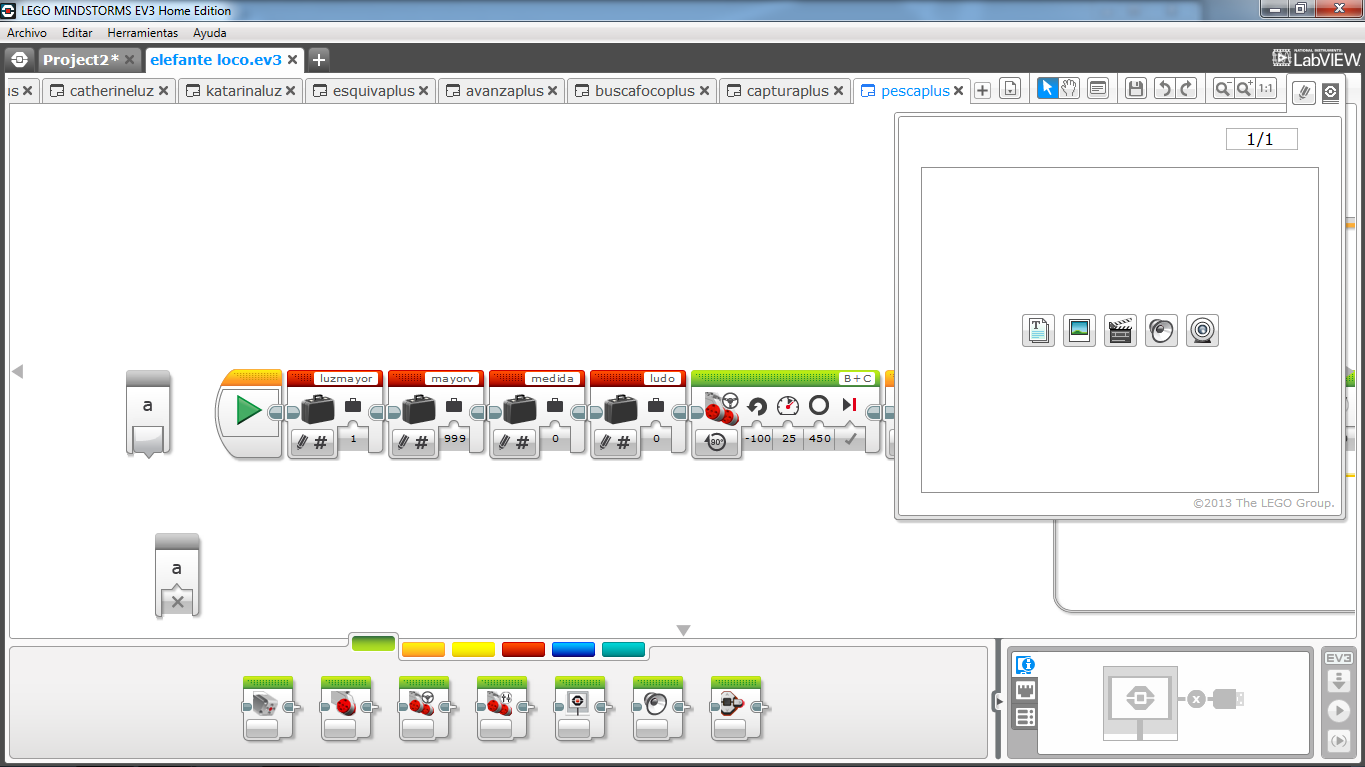
\includegraphics[width=\linewidth]{Programa.PNG}
	\centering
\end{figure}

\begin{enumerate}
\item Area de diseño del programa.
\item Sección de bloques disponibles.
\item Página de hardware.
% FIXME Que demonios es el 4?
\item Editor de contenidos.
\item Barra de herramientas.
\end{enumerate}

\subsubsection{Proyecto}

Como en la mayoría de IDES los archivos se organizan en proyectos, que pueden
contener programas experimentos imágenes y archivos de sonido. Los experimentos
son programas que crea automáticamente el IDE para capturar datos. En la figura
\ref{fig:proyecto} se puede observar los componentes de la ventana de proyecto.

\begin{figure}
	\caption{Ventana de proyecto.\label{fig:proyecto}}
	\includegraphics[width=\linewidth]{image28.jpg}
	\centering
\end{figure}

\subsubsection{Página de hardware}
Aquí muestra la información sobre el bloque EV3 que está conectado, versión de
firmware, tipo de conexión (entre el pc y el bloque), configuración inalámbrica,
barra de memoria, etc. También están las opciones de descargar programa al
brick, descargar y ejecutar o ejecutar seleccionados.

\begin{figure}[H]
	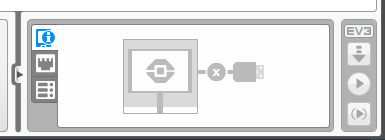
\includegraphics{controEV3.PNG}
	\centering
\end{figure}

%%%%%%%%%%%%%%%%%%%%%%%%%%%%%%%%%%%%%%%%%%%%%%%%%%%%%%%%%%%%%%%%%%%%%%%%%%%%%%%
\clearpage 
\section{Lenguaje de Programación}

\subsection{Introducción}

Los programas se crean arrastrando bloques (que tienen diferentes comportamientos
como variables control de flujo, sensores o actuadores) que representan los
elementos básicos del lenguaje. Todo programa empieza por el bloque iniciar y su
ejecución va de izquierda a derecha. Algunos bloques tienen una ejecución no
bloqueante es decir, su acción persiste mientras otro bloque posterior no la
finalice explícitamente. La ejecución finaliza cuando se llega al extremo derecho
y no hay mas bloques o explícitamente con el bloque finalizar.

\subsection{Secuencias de Bloques}

Cuando los bloques están juntos o unidos por un cable forman una secuencia de
bloques.

\begin{figure}[H]
	\includegraphics{image38.jpg}
	\centering
\end{figure}

\subsection{Secuencias Paralelas}

Cuando los bloques están en paralelo, ya sea por el bloque iniciar o a partir de
un bloque en concreto su ejecución es igual que en secuencia pero eso si, todas
las secuencias comparten las variables y en caso de conflicto su  comportamiento
es impredecible ya que solo está garantizada la ejecución atómica de cada bloque
individualmente.

\begin{figure}[H]
	\includegraphics{image39.jpg}
	\centering
\end{figure}

\subsection{Creación de bloques}

Este lenguaje fomenta la aplicación de <<funciones>> que sería lo análogo a la
creación de un bloque propio para agrupar secuencias de bloques con un
comportamiento concreto. Para ello se emplea el <<Constructor de Mi Bloque>> en el
que se definen: Nombre, icono, tipo de dato y valor por defecto para sus
respectivas entradas y salidas.

\begin{figure}[H]
	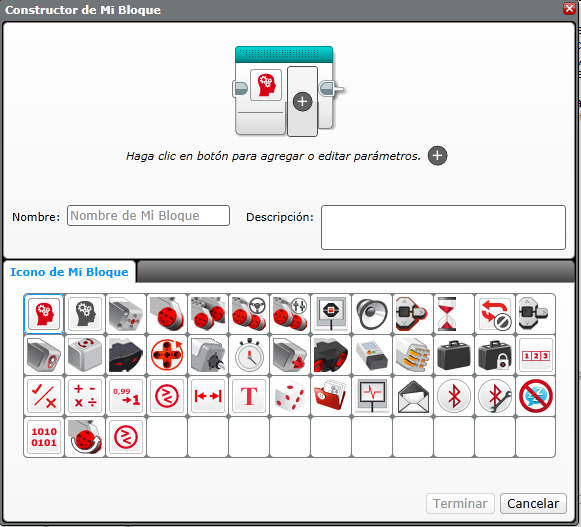
\includegraphics{ConstructorBloques.PNG} 
	\centering
\end{figure}

Una vez creados, estos bloques se pueden cambiar pero no se pueden editar ni sus
entradas ni sus salidas.

\subsection{Tipos de datos}

Existen cinco tipos de datos básicos para representar la información del
programa. Son los siguientes.

\begin{itemize}
\item Numérico
\item Lógico
\item Texto
\item Secuencia numérica
\item Secuencia lógica
\end{itemize}

El texto puede ser unicode pero la pantalla del brick solo representa los
caracteres ASCII de 7 bits. Las secuencias son arrays unidimensionales (no existe
otro tipo)

\subsection{Variables y constantes}

El lenguaje soporta los conceptos tradicionales pero son tediosas de usar.

\subsubsection{Variables}

Se usan si un dato va a ser accedido y actualizado en diferentes puntos del
programa o si se necesita un dato en diferentes secuencias (ya que se
comparten).

\subsubsection{Constantes}

Se usan si un dato solo va a ser accedido.

\subsection{Cables de datos}

Este lenguaje trata de evitar uso de variables, los cables de datos con
conexiones entre los bloques para pasar los resultados de otros bloques, es
decir son un paso por valor entre bloques. El bloque origen debe estar antes que
el bloque de destino en la secuencia y el bloque destino no se ejecuta hasta que
el dato está disponible por lo que es posible usar cables de datos para
sincronizar secuencias paralelas. Estos cables pueden pasar todos los tipos de
datos, y se puede ver su contenido durante la ejecución de un programa.

\subsection{Bloques predefinidos}

\subsubsection{Bloques de acción}

\begin{figure}[H]
	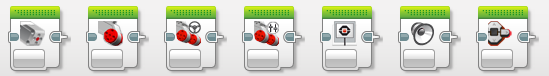
\includegraphics[width=\linewidth]{acciones.PNG}
	\centering
\end{figure}

Bloques de los motores (mediano y grande), mover la dirección, mover en tanque,
pantalla, sonido y luz de estado EV3.

\subsubsection{Bloques de control de flujo}

\begin{figure}[H]
	\caption{Bloque iniciar y bloque finalizar}
	\includegraphics{image45.jpg}
	\includegraphics{image46.jpg}
	\centering
\end{figure}

\begin{figure}[H]
	\caption{Bloque de flujo condicional if-then-else.}
	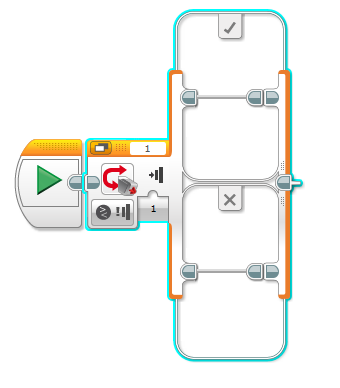
\includegraphics{condicional.PNG}
	\centering
\end{figure}

\begin{figure}[H]
	\caption{Bloque de bucle y condición para finalizar el bucle.}
	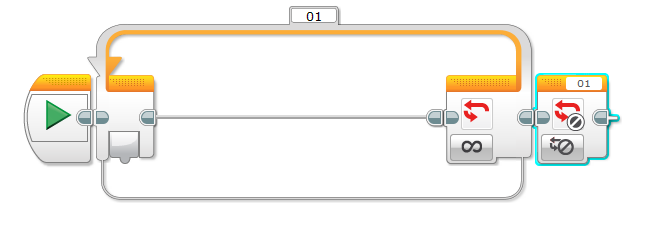
\includegraphics{bucle.PNG}
	\centering
\end{figure}

\begin{figure}[H]
	\caption{Bloque de retardo o sleep}
	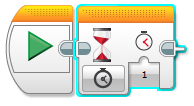
\includegraphics{sleep.PNG}
	\centering
\end{figure}

\subsubsection{Bloques de sensores}

\begin{figure}[H]
	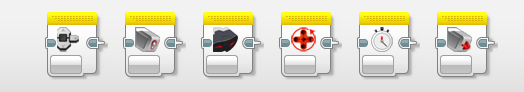
\includegraphics[scale=0.8]{sensores.PNG}
	\centering
\end{figure}

Botones del brick, sensor de color, sensor de giro, sensor infrarrojo, rotación del
motor, sensor de temperatura, temporizador, sensor táctil, sensor ultrasónico,
medidor de energía y sensor de sonido NXT.

\subsubsection{Bloques de datos}

\begin{figure}[H]
	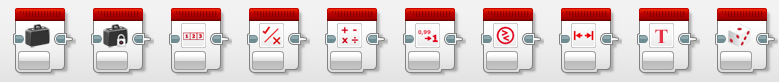
\includegraphics[scale=0.8]{operaciones.PNG}
	\centering
\end{figure}

Variable, constante, operaciones secuenciales, operaciones lógicas, matemáticas,
redondear, comparar, alcance, texto y aleatorio.

\subsubsection{Bloques de Avanzados}

\begin{figure}[H]
	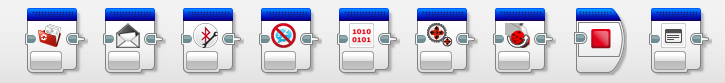
\includegraphics[scale=0.8]{avanzado.PNG}
	\centering
\end{figure}

Acceso a archivo, registro de datos, mandar mensaje, conexión bluetooth,mantener
archivo, valor del sensor sin procesar, motor sin regular, invertir el motor,
detener el programa.

\subsubsection{Mis bloques}

\begin{figure}[H]
	
\includegraphics[scale=0.8]{BloquesPersonalizados.PNG}
	\centering
\end{figure}

Aquí estarán los bloques creados.

\subsection{Flujo de un programa}

\subsubsection{Iniciar}

Marca el inicio de una secuencia de bloques ya que puede haber más de una
secuencia. Todas las secuencias se inician automáticamente cuando se inicia el
programa y se ejecutan al mismo tiempo.

\subsubsection{detener}

Finaliza una secuencia de bloques aunque su uso no es obligatorio.Finaliza todas
las secuencias en ejecución.

\subsection{E/S básica}
\subsubsection{Pantalla}
Muestra texto o gráficos.Modos de funcionamiento:
\begin{itemize}
\item Texto
\item Formas
\item Imagen
\item Reiniciar
\end{itemize}
Ejemplo de uso :
\begin{itemize}
\item Iniciar.
\item Escribir en pantalla - Borrar pantalla.
\item Esperar 2 segundos.
\item Escribir texto y no borrar la pantalla.
\item Esperar 2 segundos.
\end{itemize}
\begin{figure}[H]
	\caption{Secuencia de ejemplo de uso pantalla}
	\includegraphics[scale=0.75]{image49.jpg}
	\centering
\end{figure}
\subsubsection{Luz de estado}
Controla la luz de estado del brick puede ser un pulso continuo o con pulsos.
\begin{itemize}
\item Encendido
\item Apagar
\item Reiniciar
\end{itemize}
Ejemplo de uso :
\begin{itemize}
\item iniciar
\item esperar
\item luz de estado roja sin pulso
\item esperar
\item luz de estado naranja con pulso
\item esperar
\end{itemize}
\begin{figure}[H]
	\caption{Secuencia de ejemplo de uso luz estado }
	\includegraphics[scale=0.75]{image49.jpg}
	\centering
\end{figure}
\subsubsection{Sonido}
Reproduce sonido en el altavoz del brick, se puede ajustar el volumen y reproducir en bucle.Esta reproducción puede ser bloqueante o no bloqueante.
Modos de funcionamiento :
\begin{itemize}
\item Archivo
\item Tono
\item Nota
\item Detener
\end{itemize}
Ejemplo de uso:
\begin{itemize}
\item Iniciar
\item Sonido (archivo)
\item Sonido (tono)
\item Sonido (nota)
\item Esperar
\item Sonido (detener)
\end{itemize}
\begin{figure}[H]
	\caption{Secuencia de ejemplo de uso Sonido }
	\includegraphics[scale=0.5]{image49.jpg}
	\centering
\end{figure}
\subsubsection{Botones del Brick}
Obtiene los datos de los botones del brick.
Modos de funcionamiento:
\begin{itemize}
\item Botones (muestra botón presionado).
\item modo comparación para botones.
\end{itemize}
\begin{figure}[H]
	\caption{Bloque de botones del brick }
	\includegraphics[scale=0.25]{image55.jpg}
	\centering
\end{figure}
\subsubsection{Motores (mover la dirección)}
Se asume que el robot tiene dos motores grandes, uno para el lado derecho del vehículo y otro para el lado izquierdo.Este bloque mueve el vehículo con un valor de potencia indicado(entre -100 y 100) y una dirección deseada.
Modos de funcionamiento:
\begin{itemize}
\item Encendido.
\item Encendido por segundos.
\item Encendido por grados o rotaciones.
\item Apagado
\end{itemize}
\begin{figure}[H]
	\caption{Bloque motor dirección }
	\includegraphics[scale=0.5]{image56.jpg}
	\centering
\end{figure}
\subsubsection{Motores (mover Tanque)}
Este bloque mueve el vehículo con un valor de potencia diferente para cada motor.
Modos de funcionamiento:
\begin{itemize}
\item Encendido.
\item Encendido por segundos.
\item Encendido por grados o rotaciones.
\item Apagado
\end{itemize}

\begin{figure}[H]
	\caption{Bloque motor Tanque}
	\includegraphics[scale=0.5]{image58.jpg}
	\centering
\end{figure}

\subsubsection{Motores (motor grande y motor mediano )}
Estes bloques mueven el vehículo con un valor de potencia diferente para cada motor.Un
número positivo implica un giro en el sentido de las agujas del reloj y un
número negativo un giro en el sentido contrario al de las agujas del reloj.
Modos de funcionamiento:
\begin{itemize}
\item Encendido.
\item Encendido por segundos.
\item Encendido por grados o rotaciones.
\item Apagado
\end{itemize}

\begin{figure}[H]
    \caption{Motores mediano y grande}
    \centering
  \begin{subfigure}{0.45\linewidth}
    \centering
	\caption{Bloque motor Grande}
	\includegraphics[scale=0.5]{image61.jpg}
  \end{subfigure} %
  \begin{subfigure}{0.45\linewidth}
    \centering
	\caption{Bloque motor mediano}
	\includegraphics[scale=0.5]{image62.jpg}
  \end{subfigure}
\end{figure}

\subsubsection{Sensor de ultrasonidos}
Envía ondas de sonido de alta frecuencia y mide cuánto tarda el sonido en reflejarse de vuelta al sensor con un rango de detección de 3 a 250cm.
Modos de funcionamiento :
\begin{itemize}
\item Distancia (al objeto más cercano)
\item presencia (detecta señales de ultrasonidos de otras fuentes)
\item Para los anteriores modo existe un modo comparación con un valor especificado
\end{itemize}
\begin{figure}[H]
	\caption{Bloque sensor ultrasonidos}
	\includegraphics[scale=0.5]{image64.jpg}
	\centering
\end{figure}
\subsubsection{Sensor de infrarrojos}
Envía luz en el espectro de los infrarrojos y detecta el reflejo de esta luz en otros objetos(hasta 70cm). 
Modos de funcionamiento :
\begin{itemize}
\item Proximidad
\item Baliza(remoto)
\item Baliza(posición)
\item Para cada modo anterior existe un modo comparación respecto a un valor
\end{itemize}
\begin{figure}[H]
	\caption{Bloque sensor de infrarrojos}
	\includegraphics[scale=0.5]{image68.jpg}
	\centering
\end{figure}
\subsubsection{Sensor giroscopio}
Detecta el movimiento de rotación en un plano(máximo 400º/seg)
Modos de funcionamiento :
\begin{itemize}
\item Angulo
\item Velocidad de rotación
\item Modo comparación y a mayores un reinicio para poner la referencia a 0º
\end{itemize}
\begin{figure}[H]
	\caption{Bloque giroscopio}
	\includegraphics[scale=0.25]{image70.jpg}
	\centering
\end{figure}
\subsubsection{Sensor de color}
Detecta color o intensidad de luz.
Modos de funcionamiento :
\begin{itemize}
\item color (entre 7 colores : negro, azul, verde, amarillo, rojo, blanco, marrón y sin color)
\item intensidad de luz reflejada
\item intensidad de luz ambiente
\item Modo comparación para todos estos métodos.
\item Calibrar mínimo(intensidad de luz a 0)
\item Calibrar máximo(intensidad de luz a 100)
\item Reinicio
\end{itemize}
\begin{figure}[H]
	\caption{Bloque sensor de color}
	\includegraphics[scale=0.25]{image71.jpg}
	\centering
\end{figure}
\subsubsection{Sensor de rotación del motor}
Obtiene información de un motor de lo que esta girando o de la potencia aplicada.
Modos de funcionamiento :
\begin{itemize}
\item Rotación
\item Potencia
\item Modo comparación para estos dos últimos
\item Reinicio
\end{itemize}
\begin{figure}[H]
	\caption{Bloque sensor rotación del motor}
	\includegraphics[scale=0.25]{image74.jpg}
	\centering
\end{figure}
\subsubsection{Sensor de contacto}
Modos de funcionamiento :
\begin{itemize}
\item Estado (si está pulsado o no)
\item Modo de comparación para el anterior modo
\end{itemize}
\begin{figure}[H]
	\caption{Bloque sensor de contacto}
	\includegraphics[scale=0.25]{image77.jpg}
	\centering
\end{figure}
\subsubsection{Sensor de temperatura}
Mide la temperatura en la punta de su sonda
metálica. El sensor mide en grados Celsius (de
-20ºC a 120ºC) y Fahrenheit (de -4ºF a 248ºF)
con una exactitud de 0,1ºC.
Modos de funcionamiento :
\begin{itemize}
\item Temperatura
\item Para el modo anterior existe un modo comparación con un valor.
\end{itemize}
\begin{figure}[H]
	\caption{Bloque sensor de temperatura}
	\includegraphics[scale=0.25]{image79.jpg}
	\centering
\end{figure}
\subsubsection{Temporizador}
Obtiene tiempo de alguno de los temporizadores del brick(que son 8)
Modos de funcionamiento :
\begin{itemize}
\item Tiempo
\item Modo comparación para el tiempo
\item Reinicio
\end{itemize}
\begin{figure}[H]
	\caption{Bloque temporizador}
	\includegraphics[scale=0.5]{image81.jpg}
	\centering
\end{figure}
\subsubsection{Espera}
Modo que espera a que suceda algo antse de continuar con el siguiente bloque de secuencia
Modos de funcionamiento :
\begin{itemize}
\item Tiempo
\item Sensor
\item Mensaje(por un mensaje bluetooth de tipo especificado)
\end{itemize}
\begin{figure}[H]
	\caption{Bloque espera}
	\includegraphics[scale=0.5]{image82.jpg}
	\centering
\end{figure}
\subsection{Control de flujo}
\subsubsection{Condicionales}
Bloque interruptor, contiene dos o mas secuencias de bloques de programación(casos). Estos casos se pueden mostrar en pestañas y puede existir un caso por defecto, puede actuar como if.. else o un switch.Modos de funcionamiento:
\begin{itemize}
\item Sensor(comprobar si el valor de un sensor cumple o no una condición)
\item Lógico (True o False para una sentencia determinada)
\item Texto(compara texto)
\item Numérico(compara número)
\end{itemize}
\subsubsection{Bucles}
Repite una secuencia de bloques contenida en su interior.
Modos de funcionamiento:
\begin{itemize}
\item Ilimitado (While True)
\item Cuenta (repite número limitado de veces)
\item Tiempo (durante un tiempo especificado)
\item Lógico(hasta que una entrada logica se cumpla)
\item Sensor (Hasta que un sensor tenga un valor determinado)
\item Mensaje (Hasta que se recibe un mensaje determinado)
\end{itemize}
\subsubsection{Break}
Interrupción de un bucle, provoca la finalización de un bucle de manera anticipada. Se puede especificar que bucle quiere interrumpirse por medio de su etiqueta y desde cualquier parte del código(Muy útil para secuencias en paralelo)
\clearpage 
\section{Ejemplo de uso: Robot }
En este ejemplo veremos un robot que tiene el siguiente comportamiento : 
\begin{itemize}
\item Sale de situaciones de colisión.
\item Evita situaciones de colisión.
\item Avanza
\item Se dirige hacia la Luz.
\item recoge una caja de determinado color.
\end{itemize}
Se incluyen estas imágenes en la carpeta img/ para poder verlas con un mayor detalle, sus nombres son de la forma Robot*.png
\subsection{Controlador Global}
\begin{figure}[H]
	\caption{Controlador global robot}
	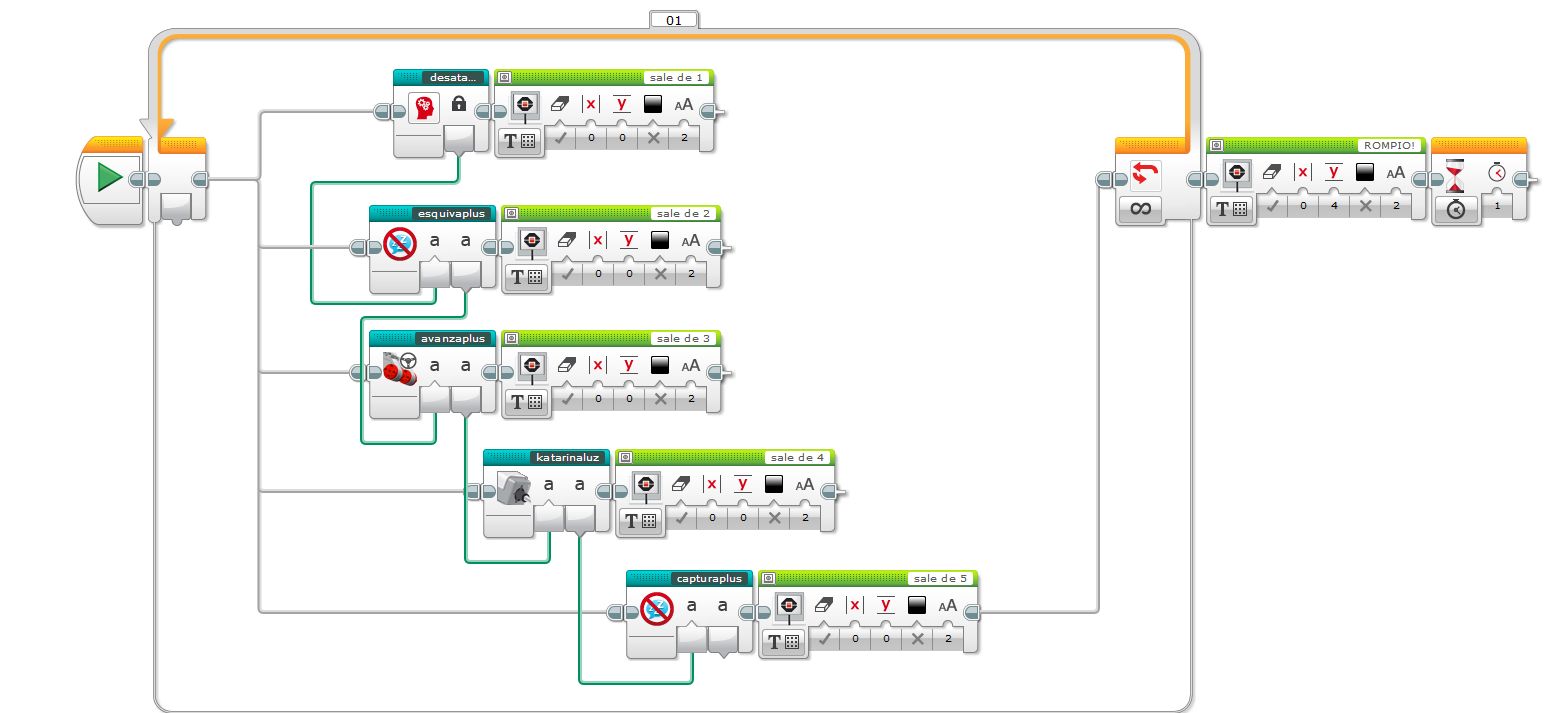
\includegraphics[scale=0.45]{RobotControladorGlobal.PNG}
\end{figure}
Se realizan de forma paralela pero controlando su ejecución con variables bool, cada modulo activa el anterior para asegurarnos unas precondiciones antes de ejecutar un determinado comportamiento.Cuando cambia de modo se imprime en la pantalla del brick.
\subsection{Salir de situaciones de Colisión}
\begin{figure}[H]
	\caption{salir de situaciones de colisión}
	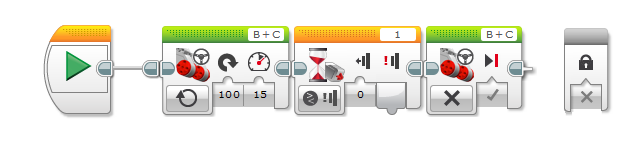
\includegraphics{RobotDesatascar.PNG}
	\centering
\end{figure}
Gira hasta que su pulsador, situado en la parte delantera es soltado, este se presionaria si el robot chocase con algo.Este comportamiento aparece muy pocas veces ya que se suelen eviar las situaciones de colisión.De ahí su sencillez.
\subsection{Evitar situaciones de colisión}
\begin{figure}[H]
	\caption{Evitar colisiones con ultrasonidos}
	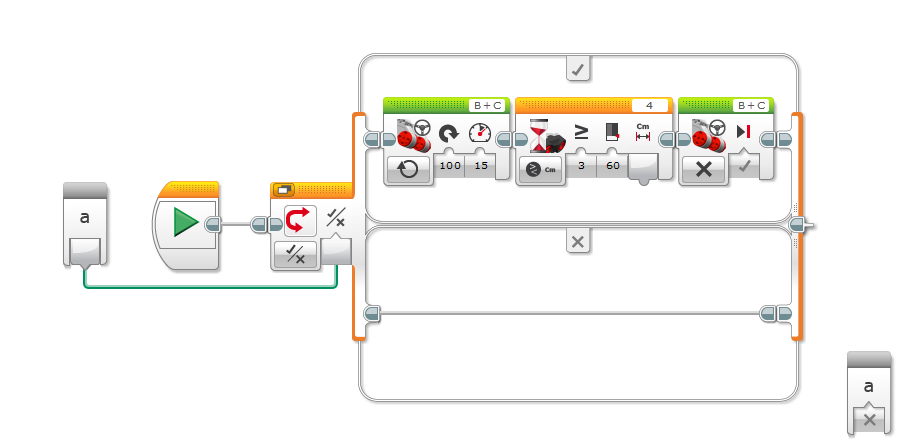
\includegraphics[scale=0.45]{RobotEsquivar.PNG}
	\centering
\end{figure}
Usa el sensor de ultrasonidos para saber a que distancia tiene la pared hacia la que está avanzando, cuando esta distancia llega a un umbral, gira.
\subsection{Avanzar}
\begin{figure}[H]
	\caption{avanzar}
	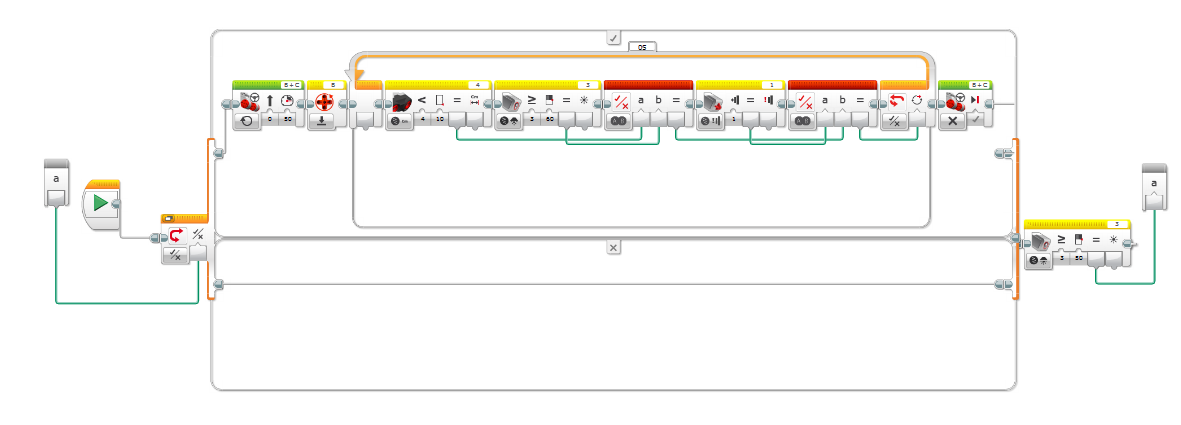
\includegraphics[scale=0.45]{RobotAvanzar.PNG}
	\centering
\end{figure}
Avanza mientras la luz no decrezca respecto a una medida anterior es decir, se esté alejando de la luz.
\subsection{Se dirige hacia la Luz}
\begin{figure}[H]
	\caption{capturar luz}
	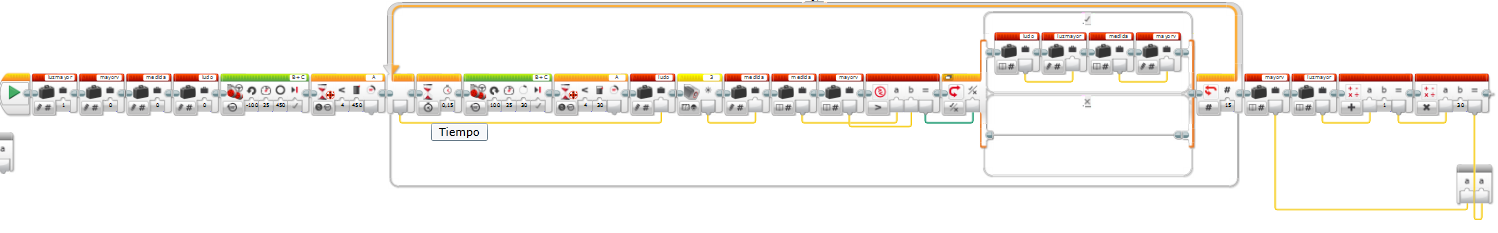
\includegraphics[scale=0.45]{RobotLuzMayorGood.PNG}
	\centering
\end{figure}
Gira hacia la luz, haciendo diferentes medidas previas.
\subsection{Recoge una caja}
Aquí diferenciamos dos comportamientos, encarar la caja y acercarse para posteriormente recogerla.
\subsubsection{Acercarse a la caja}
\begin{figure}[H]
	\caption{Acercarse a la caja}
	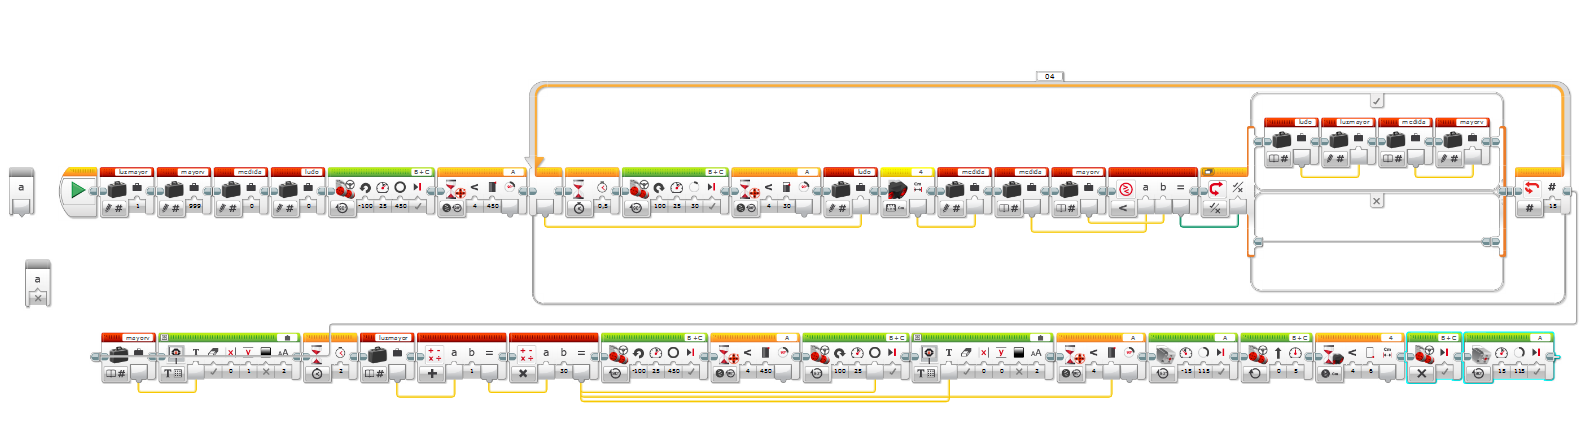
\includegraphics[scale=0.45]{RobotLuzMayorCaja.PNG}
	\centering
\end{figure}
\subsubsection{Recoger la caja} 
\begin{figure}[H]
	\caption{recoger la caja}
	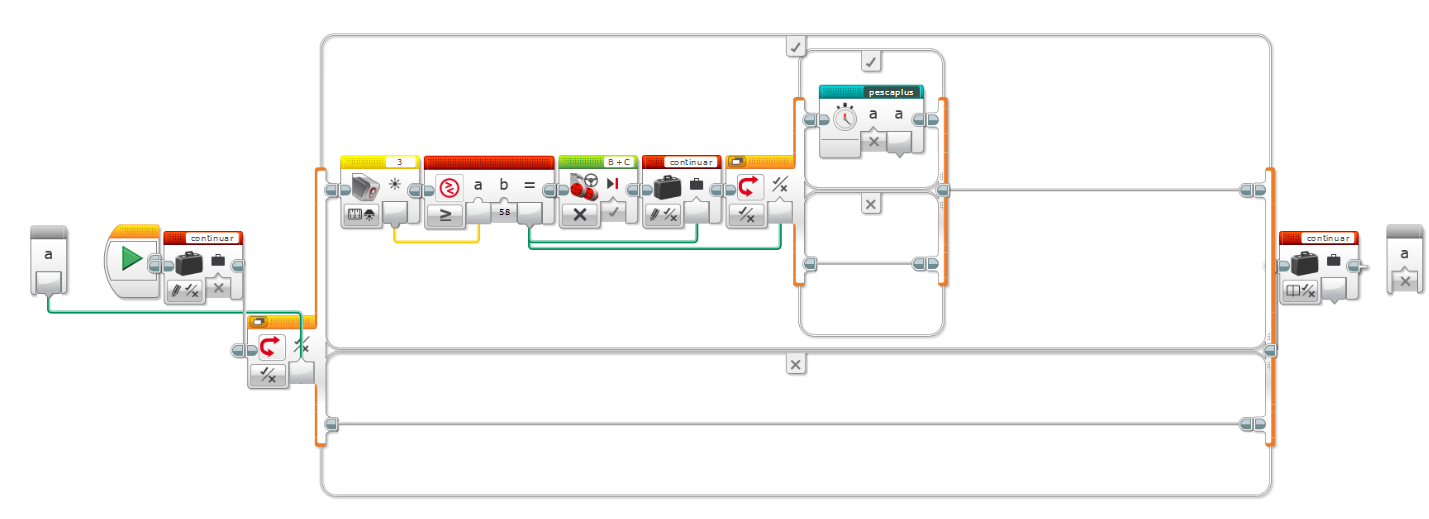
\includegraphics[scale=0.45]{RobotCapturarCaja.PNG}
	\centering
\end{figure}

\section{Comparación con lenguajes tradicionales.}
\subsection{Memoria}
En lenguajes tradicionales como Fortran, C o Pascal, es necesario reservar y 
liberar la memoria de forma manual.

Sin embargo en lenguaje de bloques de Lego, la memoria se maneja de forma 
automática. No es necesario reservar espacio explícitamente para almacenar una 
variable, y posteriormente liberarlo. De modo que incluye un recolector de 
basura para las variables que ya no se emplean.

\subsection{Intérprete}
El IDE es en realidad un compilador a un lenguaje intermedio llamado bytecode 
que es propiedad de Lego. Cada bloque es transcrito en una serie de 
instrucciones, que forman un <<clump>>. Estos fragmentos, se tratan como tareas 
indivisibles, y son las que se ejecutarán siguiendo el orden establecido por la 
máquina virtual de Lego. Para la ejecución de un <<clump>>, todos los bloques de 
los que depende, deben haberse ejecutado. Esto posibilita la paralelización de 
las ejecuciones.

\subsection{Paralelismo}
Algunos lenguajes de alto nivel, proporcionan un mecanismo sencillo para manejar 
operaciones que se realizan en segundo plano. Otros, sin embargo no incluyen 
dicha facilidad, relegando al programador la tarea de diseñar un mecanismo para 
realizar varias acciones a la vez.

En un lenguaje, donde se busca la simplicidad y facilidad de uso, el paralelismo 
se realiza de forma transparente para el usuario. De forma que los mecanismos 
para controlar que tarea se debe realizar, y de que manera se comparte el cpu 
entre tareas, quedan fuera del alcance del programador.

Para realizar una ejecución paralela, basta con emplear una bifurcación en el 
cable que conecta dos bloques, para incluir dos o mas bloques cuya conexión 
parte del mismo lugar. De esta forma cualquier bloque conectado, será ejecutado 
en paralelo.

El modo de resolver los problemas de acceso entre las variables se soluciona 
compartiendolas de forma global. Sin embargo, de forma interna, se mantiene un 
registro de todas las variables, protegidas mediante mutex, para el correcto 
funcionamiento de los bloques en paralelo.

\subsection{Funciones}
Las clásicas funciones, son ahora reemplazadas por bloques que engloban un 
funcionamiento concreto. Son aquellos creados por el mecanismo de bloques 
propios, y que realizan un conjunto de operaciones definidas en un plano aparte 
del programa. Lo que permite centrarse en la resolución de un problema, pequeño, 
y concreto.

Los argumentos de las funciones, son siempre pasados por valor, empleando las 
conexiones a unos bloques especiales.

\subsection{Recursión}
Lego Mindstorms EV3 no soporta la recursión. Sin embargo hay otros entornos como  
LeJOS EV3 (Java, gratuíto) y ROBOTC (C, no gratuíto), que sí la soportan.

\subsection{Polimorfismo}
De igual manera que lenguajes de alto nivel como Java, soportan el polimorfismo, 
el bytecode de Lego también lo hace. Sin embargo, se realiza de manera 
transparente para el usuario. Por ejemplo, en la comparación de dos enteros de 
distinto tamaño, 32 y 16 bits, se realiza previamente una conversión a tipos de 
32 bits.


\end{document}
